\documentclass[10pt]{article}
\setlength{\parskip}{0.25\baselineskip}
\usepackage[margin=1in]{geometry} 
\usepackage{amsmath,amsthm,amssymb, graphicx, multicol, array}
\usepackage[font=small,labelfont=bf]{caption}
\usepackage{float}
\usepackage{bbm}

\newcommand{\supp}{{\text{supp}}} 
\newcommand{\bv}{{\text{BV}}}
\newcommand{\ac}{{\text{AC}}}
\newcommand{\vol}{{\text{Vol}}}

\newenvironment{problem}[2][]{\begin{trivlist}
\item[\hskip \labelsep {\bfseries #1}\hskip \labelsep {\bfseries #2.}]}{\end{trivlist}}

\begin{document}
 
\title{Homework \#9}
\author{Eric Tao\\
Math 123: Homework \#9}
\maketitle

\begin{problem}{Question 1}

Download the data 'HW9\_TwoClassSeparable.mat' with data $\{ x_i \}_{i=1}^n \subset \mathbb{R}^2$ with labels $\{  y_i \}_{i=1}^n$.

(a) Use the MATLAB function 'fmincon.m' to solve the dual problem to the hard margin SVM. Then, compute the relevant hyperplane parameters and display the optimal separating hyperplane. What is the margin of the optimal hyperplane?

(b) Let $F(w,b) = \Vert w \Vert^2 + \alpha \sum_{i=1}^n \max(0,1 - y_i(w^T x_i + b))$ be the soft-margin hinge loss. Use the same function to compute the solution to the dual problem for a range of $\alpha \geq 0$, and plot the corresponding hyperplanes. Are all the hyperplanes separating? Explain.

\end{problem}

\begin{proof}[Solution]

(a) 

We recall, that solving the dual problem to the hard margin SVM is equivalent to finding $\lambda = (\lambda_1,...,\lambda_n)$ such that:

$$F( \lambda) = -\frac{1}{4} \sum_{i=1}^n \sum_{j=1}^n \lambda_i \lambda_j y_i y_j x_i^T x_j + \sum_{i=1}^n \lambda_i $$ is maximized. Equivalently, in matlab, we try to find the minimum of $-F(\lambda)$, under the constraints $\lambda_i \geq 0$ and $\sum_{i=1}^n \lambda_i y_i = 0$.

Then, we computed $$ \begin{cases} w = \frac{1}{2} \sum_{i=1}^n \lambda_i y_i x_i \\ b_{max} = \max_{y_i = 1} (1 - w^T x_i) \\ b_{min} = \min_{y_i = -1} (-1 - w^T x_i) \\ b = \frac{b_{min} + b_{max}}{2} \end{cases}$$

What we found was the following:

\begin{center}
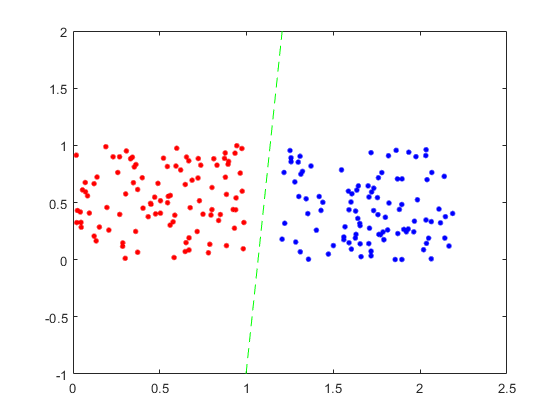
\includegraphics[width=\linewidth]{dual_hard_svm}
\captionof{figure}{Hard Margin SVM}
\end{center}

with a margin of $ \Vert w \Vert_2^2 \approx 5*10^{-4} $

(b)

In a similar fashion, solving the dual problem to the soft-margin SVM is equivalent to finding the maximum of :

$$F( \lambda) = -\frac{1}{2} \sum_{i=1}^n \sum_{j=1}^n \lambda_i \lambda_j y_i y_j x_i^T x_j + \sum_{i=1}^n \lambda_i $$

where now we have $0 \leq \lambda_i \leq \alpha$ for our bounds, and we still have that $\sum_{i=1}^n \lambda_i y_i = 0$, where we've primarily just introduced the $\alpha$ as an upper bound to the values of $\lambda$.

Doing the same computation on minimizing, for some choices of $\alpha$, we find:

\begin{center}
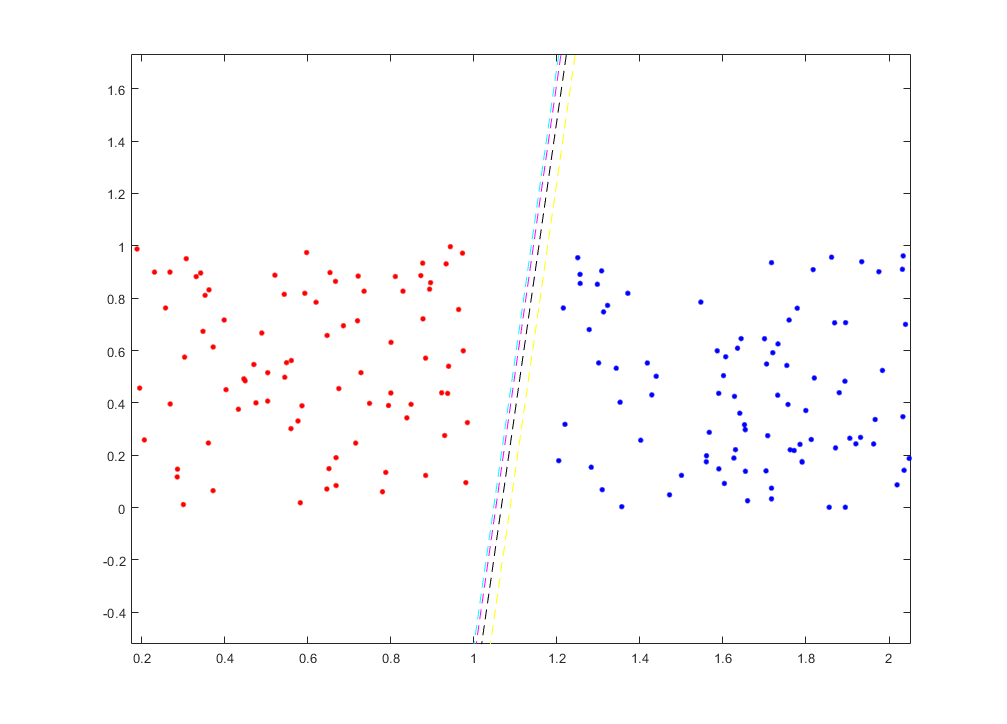
\includegraphics[width=\linewidth]{dual_soft_svm}
\captionof{figure}{Soft Margin SVM, CMYK, $\alpha = 0.1, 1,10,100$}
\end{center}

I don't really see what the distinction here, but because the data is linearly separable already, softening the margins doesn't really change much. It is somewhat interesting how each line is skewed towards one direction or another, but likely that's due to the amount of support vectors on each side.

\end{proof}

\begin{problem}{Question 2}

For labeled data $\{ (x_i, y_i) \}_{i=1}^n$, let $F(w,b) = \Vert w \Vert^2 + \alpha \sum_{i=1}^n \max(0,1 - y_i(w^T x_i + b))^2$ the the soft-margin quadratic loss.

(a) Prove that minimizing this loss is equivalent to minimizing $G(w,b,\zeta) = \Vert w \Vert^2 + \alpha \Vert \zeta \Vert^2$ subject to hard constraints $y_i (w^T x_i + b) \geq 1 - \zeta_i$. We call the variables $\zeta = (\zeta_1,...,\zeta_n)$ slack variables.

(b) Prove that the corresponding dual problem is maximized when $w = \frac{1}{2} \sum_{i=1}^n \lambda_i y_i x_i$ and $b = y_i (1 - \zeta_i) - w^T x_i $ for any $\zeta_i > 0$. 

\end{problem}

\begin{proof}[Solution]

(a)

We notice that $F,G$ only differ in the second term. Thus, we need only compare the behaviors of $\zeta$, and $\max(0,1 - y_i(w^T x_i + b))^2$. Well, we notice by the hard constraint, that:

$$ y_i (w^T x_i + b) \geq 1 - \zeta_i \implies \zeta_i \geq 1 -  y_i (w^T x_i + b)$$

and that because $\zeta$ is a vector composed of the $\zeta_i$, that $\Vert \zeta \Vert_2^2$ takes on a minimum when each $\zeta_i $ is as small as possible in absolute value. Then, looking at a minimizing set for $G$, since $\zeta_i \geq  1 -  y_i (w^T x_i + b)$ and $\Vert \zeta \Vert_2^2 = \sum_{i=1}^n \zeta_i^2$, a set of non-negative reals, $\Vert \zeta \Vert_2^2$ takes on a minimum exactly at $\zeta_i = \max\{0,1 - y_i(w^T x_i + b) \}$, as the global minimum for $\Vert \zeta \Vert_2^2$ is 0 for the zero vector, but our hard constraints may force us to take on a positive value. But, this implies that at a minimizing set, we have that $\zeta_i^2 = \max\{0,1 - y_i(w^T x_i + b) \}^2$, exactly the same term as in $F$.

(b)

Recall that the dual problem to the soft-margin SVM with quadratic loss has form:

$$g(\lambda, \mu) = \min_{w,b,\zeta} \left( \Vert w \Vert_2^2 + \alpha \Vert \zeta \Vert_2^2 -  \sum_{i=1}^n \lambda_i (y_i (w^T x_i + b) - 1 + \zeta_i) - \sum_{i=1}^n \mu_i \zeta_i \right)$$

under the constraints $\lambda_i, \mu_i \geq 0$, where all we've really done is to rewrite the $G(w,b,\zeta)$ from part (a) and introduce Lagrange multipliers for the constraints:

$$ \begin{cases} \lambda_i: y_i(w^T x_i + b) \geq 1  - \zeta_i \\ \mu_i: \zeta_i \geq 0 \end{cases} $$

Of course, if we're at a maximum for this, we must have that the gradient with respect to $w$ is 0. Well:

$$\nabla_w \cdot  \left( \Vert w \Vert_2^2 + \alpha \Vert \zeta \Vert_2^2 -  \sum_{i=1}^n \lambda_i (y_i (w^T x_i + b) - 1 + \zeta_i) - \sum_{i=1}^n \mu_i \zeta_i \right) =  0 \implies$$

$$ \nabla_w \cdot \left( \Vert w \Vert_2^2 - \sum_{i=1}^n \lambda_i y_i w^T x_i  = 0\right) \implies \sum_{i=1}^n 2w_i - \sum_{i=1}^n \lambda_i y_i x_i= 0 \implies$$

$$ 2w - \sum_{i=1}^n \lambda_i y_i x_i= 0  \implies w = \frac{1}{2}  \sum_{i=1}^n \lambda_i y_i x_i $$

as desired. Now, looking at $b$, we first compute the gradient with respect to $\zeta$. In the same way as computing the gradient with respect to $w$, we find:

$$ \nabla_\zeta \left( \alpha \Vert \zeta \Vert_2^2 - \sum_{i=1}^n \lambda_i \zeta_i - \sum_{i=1}^n \mu_i \zeta_i \right) = 0 \implies 2 \alpha \zeta - \sum_i \lambda_i  - \sum_i \mu_i = 0 \implies $$

$$ \sum_i \zeta_i = \frac{1}{2 \alpha} \left( \sum_i \lambda_i + \sum_i \mu_i \right)$$

where we view $\lambda = ( \lambda_1,...,\lambda_n)$ and same with $\mu$.

Now, using the constaints $  \zeta_i \geq 1 -  y_i (w^T x_i + b)$, we choose $i$ such that $\zeta_i$ is non-0. Such a $\zeta_i$ must exist, as if not, then $\Vert \zeta \Vert_2^2 = 0$, and $F(w,b)$ is trivially minimized at $w = 0$. Since we want to minimize this, we can say that$ \zeta_i =  1 -  y_i (w^T x_i + b)$.

Then, we have that $b$ takes on:

$$ \zeta_i =  1 -  y_i (w^T x_i + b) \implies b = y_i (1- \zeta_i ) - w^T x_i $$

under the constraint on $\zeta$ from above. 


\end{proof}

\begin{problem}{Question 3}

Consider linearly separable data $\{ (x_i, y_i) \}_{i=1}^n, x_i \in \mathbb{R}^d, y_i \in \{ -1, 1 \}$. Let $\{ x | w^T x + b = 0 \}$ be the margin-maximizing hyperplane that separates the data.

(a) Show that there are at least two support vectors, that is, points that minimize the distance between the maximum margin hyperplane and the data.

(b) Could there be more than two support vectors? If so, show an example. If not, prove why not.

\end{problem}

\begin{proof}[Solution]

(a)

This should be clear. Let $f(x)$ be the shortest distance between $H$, the hyperplane, and the point $x$. Consider the set $S_1 = \{ x_i : y_i = 1 \}$ and the set $S_{-1} = \{ x_i : y_i = -1 \}$.

Explicitly, we write:

$$f(x) = \inf_{y \in H} \sqrt{x^2 + y^2} $$

If we view this as a multivariable function $g(x,y) = \sqrt{x^2 + y^2}$, it should be clear that this is a continuous function, being the composition of two continous functions. Then, taking this to an infimum over $y$, we must have the resulting single variable function over $x$ must be continuous, by an application of the triangle inequality. Thus, $f(x)$ as stated above is a continuous function.

However, $S_1, S_{-1}$ are closed sets, being singletons, and, because they're finite, moreover, they are compact. Thus, $f$ achieves a minimum on each of $S_1, S_{-1}$, and the points that achieve the minimum can be taken as support vectors.

(b)

Of course. Suppose we sample points lying in $\mathbb{R}^2$, with $S_1 = \{ (1,t ) : t \in \mathbb{R} \}$, and $S_{-1} = \{ (-1, t) : t \in \mathbb{R} \}$. With enough points, it should be evident that the maximum margin hyperplane must be the hyperplane given by $x = 0$. However, we notice that for every point in $S_1, S_{-1}$, the distance from $x=0$, to the point is exactly $1$. Thus, every point is at a minimum distance, and thus every point is a support vector.


\end{proof}

\begin{problem}{Question 4}

Use the dual optimzation formulation to solve the following optimization problems, currently written in their primal form.

(a) Minimize $x^2 + y^2$ subject to $x \leq y, x \leq 1 - 2y$.

(b) Minimize $x^2 + y^2 + z^2$ subject to $x + y + z \geq 1$.


\end{problem}

\begin{proof}[Solution]

(a)

In the general setting, we may view our objective function as:

$$f(x) = x^T I x $$

where $x = (x,y)$, and $I$ is the $2 \times 2$ identity matrix.

Then, we identify our constaints as:

$$\begin{cases} h_1(x) = \begin{pmatrix} -1 \\ 1 \end{pmatrix} x \\ h_2(x) = \begin{pmatrix} -1 \\ -2 \end{pmatrix} x +1 \end{cases}$$

where we wish $h_i \geq 0$. 

Then, in the dual problem, we wish to find $\lambda_1, \lambda_2 \geq 0$ such that

$$g(\lambda) = -\frac{1}{4} \sum_{i=1}^2 \sum_{j=1}^2 \lambda_i \lambda_j z_i^T z_j - \lambda_2$$

is maximized. Well, since $z_1^T z_2 = -1, z_1^T z_1 = 2, z_2 ^T z_2 = 5, z_2^T z_1 = -1$: we have:

$$ g(\lambda) = -\frac{1}{4} (-2 \lambda_1 \lambda_2 + 2 \lambda_1^2 + 5 \lambda_2^2 ) - \lambda_2$$

If we look for critical points, we see:

$$\begin{cases} \frac{\partial g}{\partial \lambda_1} = -\frac{1}{4} (-2 \lambda_2 + 4 \lambda_1) = 0 \implies \lambda_2 = 2 \lambda_1 \\  \frac{\partial g}{\partial \lambda_2} = - \frac{1}{4} (-2 \lambda_1 + 10 \lambda_2) - 1 = 0 \implies  -2\lambda_1 + 10 \lambda_2 + 4 = 0\end{cases} $$ 

Which implies that:

$$\begin{cases} 18 \lambda_1 + 4 = 0 \implies \lambda_1 = -\frac{4}{18} \\ \lambda_2 = -\frac{8}{18} \end{cases} $$

Since that is outside of the constaints, we look instead at $\lambda_1 = 0, \lambda_2 = 0$. We see that on the line $\lambda_1 = 0$:

$$g_{\lambda_1 = 0)} =  -\frac{1}{4} (5 \lambda_2^2 ) - \lambda_2$$ which is maximized when $\lambda_2 = 0$, because for $\lambda_2 \geq 0$, $ -\frac{1}{4} (5 \lambda_2^2 )  \leq 0$ and $-\lambda_2 \leq 0$. It should be clear that the same happens on $\lambda_2 = 0$. Thus, the minimum happens at $\lambda_1 = \lambda_2 = 0$, and thus we have that the minimizing point happens at:

$$ x_* = \frac{1}{2} \lambda_i z_i = (0,0) $$ and our minimum value there is $0^2 + 0^2 = 0$, as expected.

(b)

Similarly, in the geneal setting, we view our objective as: $$f(x) = x^T I x$$

where $x = (x,y,z)$ and $I$ is the $3 \times 3$ identity matrix.

Then, we identify our single constaint as:

$$ h_1 =  \begin{pmatrix} 1 \\ 1 \\ 1 \end{pmatrix}x - 1$$

where we wish $h_1 \geq 0$.

In the dual problem, we wish to find $\lambda$ such that:

$$ g(\lambda) = -\frac{1}{4} (3 \lambda^2) + \lambda$$

is maximized. Taking a derivative, we see:

$$\frac{\partial g}{\partial \lambda} = -\frac{3}{2} \lambda + 1 = 0 \implies \lambda = \frac{2}{3} $$

Then, we have that our ideal minimum is at:

$$ x_* = \frac{1}{2} \lambda   \begin{pmatrix} 1 \\ 1 \\ 1 \end{pmatrix} =  \begin{pmatrix} 1/3 \\ 1/3 \\ 1/3 \end{pmatrix}$$

and therefore, we have a minimum value of:

$$x^2 + y^2 + z^2 =  3 * \frac{1}{3}^2 = \frac{1}{3} $$

\end{proof}


\end{document}